\chapter{Watermark Evidence Framework}\label{cpt:evidence-framework}

This chapter instantiates the evidence contract from Eq.~\ref{eq:lifecycle-stage} for the first access-model break in the lifecycle. It first asks what can be recovered under the strongest evaluated access model: admitted local white-box code models with inspectable program carriers. It then asks what evidence remains when that access disappears behind a provider API. The contrast is central to the thesis: a strong white-box provenance mechanism and a sparse black-box audit signal should not be forced into the same claim type. Both stages use fixed denominators, negative controls, and explicit forbidden interpretations.

\section{Shared Evidence Model}

All modules in the dissertation distinguish claim-bearing rows from support-only rows. A claim-bearing row is a record whose task identifier, model or provider, prompt hash, output hash, detector version, threshold version, control status, decision rule, and score field are fixed before it enters the main denominator. The observed decision value is evaluated only after admission. Support-only rows may be useful for debugging, canary checks, stress exploration, or appendix examples, but they are not allowed to change the numerator or denominator of the main result.

The shared record abstraction is
\begin{equation}
  r_i=(u_i,a_i,h^p_i,h^{raw}_i,h^{struct}_i,v_D,v_\tau,c_i,d_i,s_i,b_i),
  \label{eq:claim-row}
\end{equation}
where $u_i$ identifies the task or case, $a_i$ identifies the access context such as model, provider, owner, or source group, $h^p_i$, $h^{raw}_i$, and $h^{struct}_i$ are prompt, raw-payload, and structured-payload hashes when applicable, $v_D$ and $v_\tau$ are detector and threshold versions, $c_i$ is the control or attack condition, $d_i$ is the decision, $s_i$ is the score or support statistic, and $b_i\in\{0,1\}$ marks whether the row is claim-bearing for its own lifecycle stage. Fields that are not meaningful for a specific module are stored as $\bot$ rather than removed, so every row still has a fixed schema.

Rows can be excluded before interpretation, but a diagnostic row cannot be promoted after its outcome is known. More explicitly, each module defines an admission predicate $\mathrm{Adm}_j(a_i,v_D,v_\tau,u_i,c_i)$ that depends on pre-outcome metadata such as model or provider context, detector version, threshold version, task identity, and control family. The claim-bearing flag is fixed by this predicate:
\begin{equation}
  b_i^{(j)} := \mathbf{1}[\mathrm{Adm}_j(a_i,v_D,v_\tau,u_i,c_i)=1].
\end{equation}
The main denominator is therefore
\begin{equation}
  \mathcal{D}_{main}^{(j)}=\{r_i:b_i^{(j)}=1,\ \mathrm{stage}(r_i)=j\}.
\end{equation}
The predicate is not allowed to depend on the observed decision $d_i$ or score $s_i$. This is the formal protection against outcome-dependent pruning; the flag records a pre-outcome admission decision rather than a label assigned after seeing results.

\begin{figure}[htbp]
  \centering
  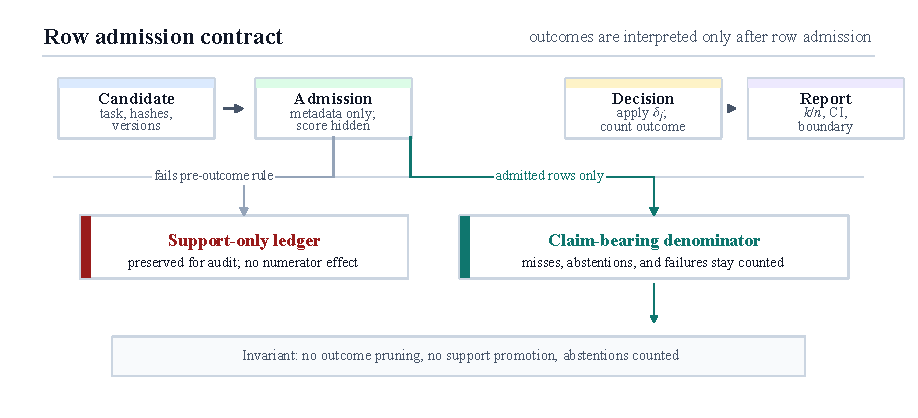
\includegraphics[width=0.96\textwidth]{fig/evidence_contract_stack.pdf}
  \caption{The row-admission contract used throughout WatermarkScope. Claim-bearing rows pass pre-outcome admission; diagnostic rows remain preserved but non-promoting.}
  \label{fig:evidence-contract-stack}
\end{figure}

\begin{algorithm}[htbp]
\caption{Evidence Admission and Claim Boundary Protocol}
\label{alg:evidence-admission}
\begin{algorithmic}[1]
\Require Candidate row $r_i$, stage $j$, frozen admission rule $\mathrm{Adm}_j$, frozen decision rule $\delta_j$
\State Bind task/case id, access context, hashes, versions, control role, and artifact path
\If{$r_i$ fails pre-outcome admission under $\mathrm{Adm}_j$}
  \State Mark $r_i$ support-only with an exclusion reason; \Return non-claim evidence
\EndIf
\State Set $b_i\gets 1$ and lock $r_i$ into denominator $\mathcal{D}^{(j)}_{\mathrm{main}}$
\State Evaluate $d_i \gets \delta_j(r_i)$
\If{$d_i$ is abstain, reject, miss, no-signal, or needs-review}
  \State Record the non-success outcome; the row remains inside $\mathcal{D}^{(j)}_{\mathrm{main}}$
\EndIf
\State Add to the numerator only when $d_i$ matches the predeclared event
\State Report $k/n$, uncertainty, support-only exclusions, and forbidden interpretations
\end{algorithmic}
\end{algorithm}

Algorithm~\ref{alg:evidence-admission} does not prove that a detector is correct. It defines when a row may support a claim and when it must remain support-only. This is why the dissertation can report strong SemCodebook recovery, sparse CodeDye signals, perfect scoped ProbeTrace attributions, and high-abstention SealAudit triage without collapsing them into one misleading score.

For example, a canary row with complete hashes can still be support-only if it was generated for a diagnostic prompt outside the frozen live denominator. Excluding that row is not cherry-picking when the exclusion was determined before seeing its decision. It would become cherry-picking only if the row were promoted because it made the numerator look better. This distinction is important for CodeDye and SealAudit, where support rows remain valuable for auditability but cannot change the main result.

For a result with $k$ observed events over $n$ claim-bearing records, the observed rate is
\begin{equation}
  \hat{p} = \frac{k}{n}.
\end{equation}
When reporting uncertainty, the dissertation uses Wilson-style confidence intervals~\cite{wilson1927probable}; the formula and zero-event convention are given in Appendix~\ref{app:artifact-index}, Table~\ref{tab:stat-reporting-rules}. These intervals are row-level descriptive intervals over admitted rows, not cluster-adjusted generalization intervals across future models, providers, owners, or tasks; clustered support surfaces are separately marked by task, model family, language, or attack family.

\section{SemCodebook: White-Box Provenance}

SemCodebook is the response to the benchmark's robustness--utility lesson: it changes the evidence object from a surface detector score to a recoverable structured identifier. It is designed for admitted white-box family and scale cells. Its goal is not merely to detect that some signal exists, but to recover a structured provenance identifier under semantic-preserving transformations. The implementation uses named rewrite/carrier families whose metadata are backed by AST-, CFG-, and SSA-style evidence. The report groups those implementation families by structural level:
\begin{equation}
  C(x) =
  \bigsqcup_{r\in\{\mathrm{AST},\mathrm{CFG},\mathrm{SSA}\}}
  \{(r,z): z\in C_r(x)\},
  \label{eq:carrier-extraction}
\end{equation}
where $\bigsqcup$ denotes a tagged disjoint union over structural evidence levels rather than a claim that the code contains only three literal carrier types. This notation is important because an AST-backed rewrite, a CFG-backed rewrite, and an SSA-style data-flow rewrite are not interchangeable even if their textual realization overlaps.
The carrier families play different roles. AST-backed carriers capture syntactic structure that survives many formatting and naming changes. CFG-backed carriers capture execution-order structure and therefore help when local syntax is rewritten but control dependencies remain recognizable. SSA-style carriers capture data-flow support, which is useful when expression-level changes preserve value dependencies. The method does not assume that every carrier family is available in every artifact; it assumes that carrier availability is measured and that insufficient support causes abstention instead of silent fallback.

A useful way to read SemCodebook is as a recovery protocol rather than as a decorative marker. The embedder chooses where the evidence may live, the executable harness checks whether the modified program remains valid, and the detector attempts to recover a provenance identifier under the same typed schedule. A row can therefore fail by missed recovery, support-gate rejection, carrier insufficiency, helper/compiler failure, or negative-control firing. All of these outcomes are more informative than a detector-only pass/fail result. The implementation schedule is adaptive: carrier families are first scored for applicability, then ranked by a frozen mixture of applicability, family prior, and keyed tie-breaking. A compact mathematical abstraction of that implementation is
\begin{align}
  q_f(x,K) &= \alpha\,a_f(x)+\beta\,b_f+\gamma\,u_f(K),\\
  \sigma_K(x) &= \mathrm{TopSlots}\bigl(\mathrm{sort}_{q_f}(F_x)\bigr),
  \label{eq:keyed-schedule}
\end{align}
where $F_x$ is the set of implementation carrier families considered for artifact $x$, $a_f(x)$ is measured applicability, $b_f$ is a frozen family bias, and $u_f(K)$ is the HMAC-derived tie-break value for the carrier key. The submitted implementation uses the resulting schedule to choose data slots and an anchor slot; Eq.~\eqref{eq:keyed-schedule} is therefore a faithful abstraction of the code path, not a second independent algorithm.
If no carrier family is applicable, or the family coverage is below the recovery threshold after row admission, the detector abstains and the outcome remains inside the positive denominator. By contrast, pre-run failures such as an unavailable model revision, missing parser, or missing helper/dependency closure produce a nonpromotion audit before the row enters the denominator. Encoded bit positions are assigned to scheduled implementation families; if the selected family has no admissible carrier, the row abstains instead of being silently moved to another family.
The carrier schedule is fixed before the checksum is formed:
\begin{equation}
  \kappa = H(\mathrm{payload}\Vert \sigma_K(x)\Vert v_{\mathrm{sched}}).
\end{equation}
The public schedule digest record is
\begin{equation}
  \mathrm{schedule\_digest}=H(K_{\mathrm{pub}}\Vert t\Vert \sigma_K(x)\Vert \kappa).
\end{equation}
Here $v_{\mathrm{sched}}$ is the frozen schedule/recovery protocol version, and $K_{\mathrm{pub}}$ is a public digest salt or verification key rather than the embedding secret $K$; the dissertation uses the digest for version binding and traceability, not as a cryptographic hiding commitment.
The watermark payload is then decoded through an ECC-style schedule block:
\begin{equation}
  \mathbf{c} = \mathrm{ECC\_Encode}(\mathrm{payload}).
\end{equation}
The schedule digest and positive-support certificate are recorded as row-level validation evidence. ECC failure, decoded-payload mismatch, incomplete positive-support evidence, and schedule-support insufficiency are counted as reject, abstain, or miss outcomes in the positive denominator, not removed from the result.
At detection time, each scheduled carrier yields a soft observation $o_i \in \{0,1,\mathrm{erasure}\}$, and the recovered payload candidate is
\begin{equation}
  \widehat{\mathrm{payload}} = \mathrm{ECC\_Decode}(o_1,\ldots,o_L).
\end{equation}
Recovery is accepted only when the decoded payload matches the expected identifier and the positive-support and schedule-commitment evidence are valid under the frozen detector version. A decoded candidate without that supporting evidence is counted as a reject, abstain, or miss, not as a recovery.

The full embed and recover pseudocode is moved to Appendix~\ref{app:reproducibility} so that the main body can keep the lifecycle argument visible. Operationally, SemCodebook has four phases: extract typed carrier evidence, schedule implementation families with a frozen key, materialize only executable-preserving carriers, and recover an identifier only when ECC-style decoding, payload matching, schedule commitment, and positive-support evidence agree. Failed materialization, insufficient carriers, ECC rejection, decoded-payload mismatch, and support-gate failure remain inside the appropriate admitted denominator rather than being removed after the fact.

The current SemCodebook evidence surface contains 72,000 structured white-box records across 10 admitted models and 5 model families. The positive detector surface contains 23,342 recoveries over 24,000 claim-bearing positives, or 97.26\%. The negative-control surface contains 0 hits over 48,000 controls. The current ablation surface contains 43,200 generation-changing rows. Table~\ref{tab:semcodebook-results} summarizes the claim-safe result.

This is the largest positive recovery surface in the dissertation under the strongest evaluated access model: local white-box code models with typed carrier inspection and executable admission. The pooled rate is used as the main-body headline only. The claim-bearing artifact records per-model, per-family, per-language, and per-attack intervals separately, and those cell-level summaries are required for any final paper table. This prevents a large or easy cell from silently dominating the interpretation.

An admitted SemCodebook cell must satisfy four pre-run conditions: the model is a local white-box code model with a frozen revision, the source group has executable tests, the language parser and carrier extractor are available, and the helper/dependency closure can be validated. The full gate table is in Appendix~\ref{app:reproducibility}, Table~\ref{tab:sem-admission-app}. A failed parser, missing helper closure, or unavailable model revision produces a nonpromotion audit rather than a smaller denominator.

\begin{table}[htbp]
\centering
\caption{SemCodebook claim-bearing denominators and control surface. Structured-row and ablation-row counts are coverage/support evidence and do not alter the recovery denominator.}
\label{tab:semcodebook-results}
\compacttable
\begin{tabularx}{\textwidth}{@{}L{2.85cm}L{2.25cm}Y@{}}
\toprule
Quantity & Value & Interpretation \\
\midrule
Recoveries & 23,342/24,000 & 97.26\%; 95\% CI about 97.04--97.46\% \\
Miss/abstain/reject & 658/24,000 & Included in positive denominator \\
Neg. control hits & 0/48,000 & 0 observed; 95\% upper bound about 0.008\% \\
Coverage/support & 72,000; 43,200 & Structured records and ablation rows; support evidence only \\
\bottomrule
\end{tabularx}
\end{table}

\begin{figure}[htbp]
  \centering
  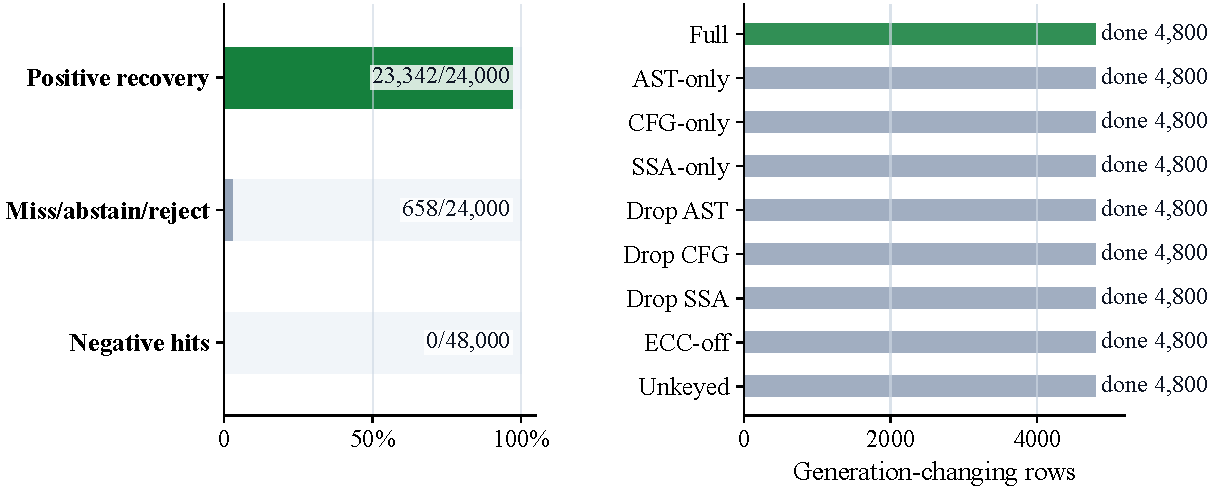
\includegraphics[width=0.96\textwidth]{fig/semcodebook_ablation.pdf}
  \caption{SemCodebook claim surface and ablation coverage. The figure separates main claim evidence from support-only ablation coverage, preserving the denominator boundary used throughout WatermarkScope.}
  \label{fig:semcodebook-ablation}
\end{figure}

The allowed SemCodebook claim is therefore rate-bound and scoped: it achieves the reported recovery and control rates within admitted white-box family and scale cells. The result also explains why the next stage is necessary. This is the first major access-model break in the dissertation. Once the model is accessed only through a provider API, the auditor can no longer inspect carrier families, helper closure, or ECC recovery state. The evidence object must change from a recoverable structural identifier to a preserved black-box transcript. This access-model break is the reason CodeDye is framed as null-audit rather than as a weaker version of SemCodebook.

The ablation design is important for scientific interpretation. The dissertation uses the promoted 43,200-row ablation gate as evidence that the major component interventions were executed under a fixed design: full AST/CFG/SSA/ECC/keyed scheduling, three single-family arms, three drop-family arms, ECC-off, and unkeyed scheduling. The ablation is reported as a promotion gate because the compact artifact binds arm counts and hash evidence; full per-arm rates remain artifact-level evidence. This keeps the main body honest: it shows that the causal questions were instrumented without inventing unsupported effect sizes in the report.

\section{CodeDye: Conservative Black-Box Null-Audit}

When carrier access disappears behind a provider API, the evidence object changes from recovery to transcript preservation. CodeDye implements this black-box audit stage. In this setting, the auditor cannot inspect model weights, carriers, helper closure, or training data. The protocol therefore records evidence rather than forcing a strong contamination claim. The implementation distinguishes a statistics-artifact signal definition from the final reporting signal: the statistics artifact records 4/300 rows under one narrow definition, while the final frozen reporting surface records 6/300 sparse audit signals. They are reported separately and are not combined. A CodeDye audit record is the black-box projection of Eq.~\ref{eq:claim-row}:
\begin{equation}
  \tilde{r}_i = (t_i, h^{p}_i, h^{raw}_i, h^{struct}_i, \mathbf{g}_i, v_D, v_{\tau}),
\end{equation}
where $\tilde{r}_i$ is the black-box projection of the full row schema: omitted fields are inherited as $c_i$, $d_i=\mathrm{signal}^{report}_i$, $s_i$ records the staged evidence summary, and $b_i=1$ only for admitted live rows. Here $h^{p}_i$ is the prompt hash, $h^{raw}_i$ is the raw response hash, $h^{struct}_i$ is the structured payload hash, $\mathbf{g}_i$ is the frozen detector gate vector, and $v_D$ and $v_{\tau}$ identify detector and threshold versions. Earlier design notes used a schematic linear score, but the claim-bearing frozen protocol uses a non-weighted familywise gate. This avoids hiding a failed evidence channel behind a high score from another channel. Let
\begin{equation}
  \mathbf{g}_i=(g^{fam}_i,g^{struct}_i,g^{direct}_i,g^{weak}_i,g^{ctx}_i)\in\{0,1\}^5
\end{equation}
record family observation, structural or stable witness evidence, direct canary evidence, weak canary evidence, and heldout/rewrite context evidence. Hash retention and chronology fields are admission/audit metadata for the row; the detector-stage reporting event is the implementation evidence stage:
\begin{align}
  \mathrm{signal}^{report}_i
  = \mathbf{1}\bigl[\mathrm{stage}(\mathbf{g}_i,\mathrm{witness}_i,\mathrm{density}_i)=4\bigr].
\end{align}
All thresholds and predicate components are fixed by the detector and threshold versions before a claim-bearing run.
The narrower statistics-artifact predicate is denoted $\mathrm{signal}^{stats}_i$ and is stored under a different threshold version:
\begin{equation}
  \mathrm{signal}^{stats}_i =
  \mathbf{1}[s^{stats}_i \geq \tau_{stats} \wedge \mathrm{hashes\_valid}_i].
\end{equation}
The numerator event uses $\mathrm{signal}^{report}_i$ only, and the denominator remains the admitted 300 live rows. The two predicates are not added together.

Appendix~\ref{app:reproducibility}, Table~\ref{tab:protocol-sketches}, gives the frozen null-audit decision sketch. In the main text, the important point is the non-weighted gate: family evidence, structural or stable witness evidence, canary evidence, and context evidence must support the final evidence stage before a row is reported as a sparse signal. A failure after row admission remains a no-signal or failure inside the 300-row denominator.

The current DeepSeek live claim surface contains 300 rows. CodeDye observes 6 sparse audit signals over those 300 rows, or 2.00\%. Positive contamination controls fire in 170/300 cases, while negative controls show 0/300 hits. In addition, 806 support rows are explicitly excluded from the main denominator. Table~\ref{tab:codedye-results} summarizes the result.

\begin{table}[htbp]
\centering
\caption{CodeDye live audit, controls, and support-row exclusions. The live signal is sparse audit yield, not prevalence.}
\label{tab:codedye-results}
\compacttable
\begin{tabularx}{\textwidth}{@{}L{2.45cm}L{2.00cm}Y@{}}
\toprule
Quantity & Value & Interpretation \\
\midrule
Live rows & 300 & Main claim denominator \\
Sparse live signals & 6/300 & 2.00\%; 95\% CI about 0.92--4.29\% \\
Positive controls & 170/300 & 56.67\%; 95\% CI about 51.0--62.2\% \\
Neg. control hits & 0/300 & 0 observed; 95\% upper bound about 1.26\% \\
Excluded support rows & 806 excluded & Retained for auditability; all excluded from the live denominator before interpretation \\
\bottomrule
\end{tabularx}
\end{table}

The intervals in Table~\ref{tab:codedye-results} are row-level Wilson intervals over admitted rows. They are not provider-general guarantees, and zero observed negative hits should be read with the printed upper bound rather than as zero false-positive risk.

The correct interpretation is a curator-side null-audit. The result is intentionally not written as contamination prevalence, provider accusation, or high-recall detection. A sparse live signal means that the frozen non-weighted evidence stage fired under the submitted audit predicate, but a no-signal row is not proof that the provider never saw related material. The value of the protocol is that it preserves evidence and prevents a weak black-box signal from being inflated into a stronger claim.

This conservative treatment is essential for academic integrity. A black-box provider response can be affected by prompt wording, retrieval-like behavior, decoding variation, and hidden moderation or safety layers. CodeDye therefore treats positive controls and negative controls as calibration evidence, while the live 6/300 signal is reported only as sparse audit yield.

This leaves one final gap. A preserved transcript can support an audit trail, but it still does not identify which registered source or owner can claim the evidence, and it does not say whether acting on the evidence is safe. Chapter~\ref{cpt:attribution-triage} therefore adds two governance layers rather than another detector: ProbeTrace binds evidence to a pre-registered owner under false-owner controls, and SealAudit routes marker-hidden risk without unsafe pass-through. Both stages keep the same denominator discipline introduced here.

This handoff defines the chapter's role in the lifecycle. SemCodebook shows what is possible when the defender can use program structure and local model access; CodeDye shows what remains defensible after those assumptions disappear. The shared contribution is not that both stages optimize the same metric. It is that both stages use the same evidence rule: the row is admitted before the result is known, controls are reported with the result, and the strongest claim is limited by the available evidence object. The next chapter applies that rule to two questions that arise only after evidence exists: who can claim it, and whether it should trigger security review.

This distinction is the main methodological bridge from watermarking to governance. A recoverable identifier answers a provenance question, while a preserved transcript answers an audit question. Neither, by itself, decides ownership or safety. The next stage therefore does not try to inflate CodeDye's sparse signal or reinterpret SemCodebook's white-box recovery as black-box detection. It adds the missing assumptions explicitly: an owner registry for attribution and a marker-hidden evidence vector for triage.
